## Recursividad: Series {.fragile}

\bgnblockgood
\strongText{Ejemplo 6:} Determine la suma de: $1 + 2 + 3 + 4 + \ldots + n$.
\trmblockgood

\pause

\begin{lstlisting}[style=frame02]
# suma1n: int -> int
# Calcula la suma de los primeros n números naturales.
# Ejemplo: suma1n(3) retorna 6
def suma1n(n):
    if n == 1:
        return 1
    else:
        return n + suma1n(n - 1)
# Tests
assert suma1n(1) == 1
assert suma1n(6) == 21
\end{lstlisting}

## Recursividad: Series {.fragile}

\bgnblockgood
\strongText{Ejemplo 7:} Calcule el valor de: $\quad\sum\limits_{0}^n \frac{1}{2^n}$
\trmblockgood

\pause

\begin{small}
\begin{lstlisting}[style=frame02]
# unMedioCeroN: int -> num
# Calcula el valor de la serie cuyo término enésimo es 1/(2^n),
# partiendo desde 0.
# Ejemplo: unMedioCeroN(5) retorna 1.96875
def unMedioCeroN(n):
    if n == 0:
        return 1
    else:
        return (1 / (2.0**n)) + unMedioCeroN(n - 1)
# Tests
assert unMedioCeroN(1) == 1.5
assert unMedioCeroN(6) == 1.984375
\end{lstlisting}
\end{small}

## Recursividad: Series {.fragile}

\bgnblockgood
\strongText{Ejemplo 8:} Calcule el valor de: $\quad\sum\limits_{1}^n \frac{1}{2^n}$
\trmblockgood

\pause

\begin{small}
\begin{lstlisting}[style=frame02]
# unMedioUnoN: int -> num
# Calcula el valor de la serie
# cuyo término enésimo es 1/(2^n),
# partiendo desde 1.
# Ejemplo: unMedioUnoN(5) retorna 0.96875
def unMedioUnoN(n):
    if n == 1:
        return 1/2.0(*@\tikzmark{markBgnHalf}@*)
    else:
        return (1 / (2.0**n)) + unMedioUnoN(n - 1)
# Tests
assert unMedioUnoN(1) == 0.5
assert unMedioUnoN(6) == 0.984375
\end{lstlisting}
\end{small}

\drawTikZComment[above right=-0.2em and 7em of markBgnHalf, text width=10em]{markBgnHalf}{\scriptsize Ojo, acá el primer valor es $\mathbf{\frac{1}{2}}$}

## Recursividad: Torres de Hanói {.fragile}

- Es un puzzle/juego matemático.
- Consiste en varios discos de distinto tamaño y tres torres.
- La idea es que todos los discos, que inicialmente están en la torre
izquierda, hay que moverlos hasta la torre derecha, respetando las siguientes reglas:
    1. Sólo un disco puede ser movido cada vez.
    1. Un disco sólo puede ser movido sobre una torre vacía o sobre otro disco más grande.

\centering    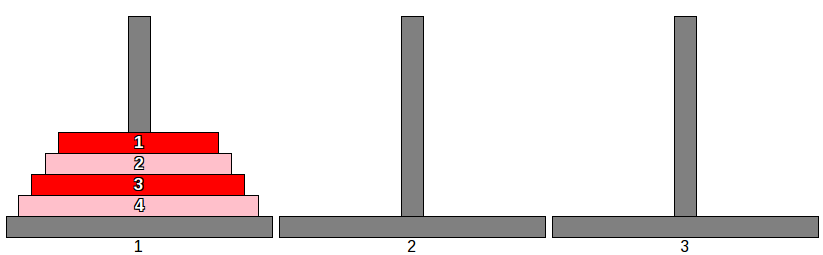
\includegraphics[width=.8\textwidth]{img/towersHanoi.png}

## Recursividad: Torres de Hanói {.fragile}

- Nuestro objetivo es saber cuántos son los pasos mínimos para resolver el juego, dados
$n$ discos.
- También se quiere determinar la mejor secuencia de pasos para resolverlo.

- Se puede ver una demostración interactiva en: \url{https://nozimica.github.io/hanoi/}

